\section{Задача C. Школьная демократия}

\begin{frame}[t]{Задача С. Школьная демократия}

  \begin{center}
    \LARGE Задача C. Школьная демократия
  \end{center}
  \begin{center}
	  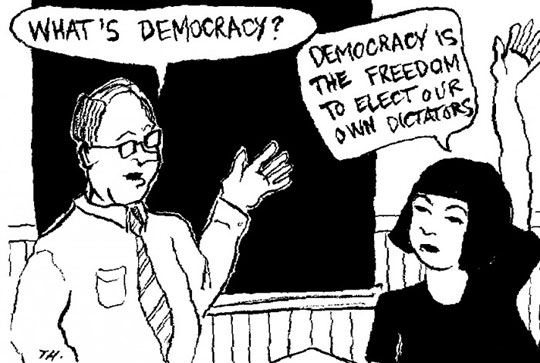
\includegraphics[width=7cm]{pics/democracy2.jpg}
  \end{center}
\end{frame}

\begin{frame}[t]{}
  \vspace{3cm}

  \begin{itemize}
    \item Идея задачи --- Евгений Курпилянский
    \item Подготовка тестов --- Евгений Курпилянский
    \item Разбор задачи --- Евгений Курпилянский
  \end{itemize}
\end{frame}

\subsection{Постановка задачи}

\begin{frame}[t]{Постановка задачи}
\begin{itemize}
  \item Дана последовательность чисел $a_1, \ldots, a_n$ ($a_i = b_i - g_i$).
  \item Требуется разбить её на отрезки длины от $l$ до $r$ так, чтобы
  {\bf разность} количества отрезков с положительной суммой и
  количества отрезков с отрицательной суммой была {\bf максимальна}.
\end{itemize}
\end{frame}

\subsection{Решение задачи}

\begin{frame}[t]{Решение задачи за $O(n^2)$}
\begin{itemize}
  \item $sum_i = a_1 + \ldots + a_i$
  \item $res_i$ --- ответ для префикса длины $i$
  \item $res_i = \max\limits_{k=l..r} \left(res_{i - k} + sign(sum_i - sum_{i - k})\right)$,
  где \[
      sign(x)= 
      \begin{cases}
         1, & \text{if } x > 0\\
         0, & \text{if } x = 0\\
        -1, & \text{if } x < 0
      \end{cases}
      \]
\end{itemize}
\end{frame}

\begin{frame}[t]{Оптимизация пересчета значений динамики}
$res_i = \max\limits_{k=l..r} \left(res_{i - k} + sign(sum_i - sum_{i - k})\right)$
\begin{itemize}
  \item Рассмотрим $X = \max\limits_{k=l..r} res_{i-k}$
  \item Заметим, что $res_i \geqslant X - 1$
  \item Если максимум достигается при $k=z$, тогда $res_{i-z} = X$ или $res_{i-z} = X - 1$
  \item Тогда $res_i = \max(A, B)$, где

        $A = \max\limits_{\substack{k=l..r\\
                                    res_{i-k}=X}} \left(X + sign(sum_i - sum_{i-k})\right)$
        
        $B = \max\limits_{\substack{k=l..r\\
                                    res_{i-k}=X-1}} \left(X-1 + sign(sum_i - sum_{i-k})\right)$
\end{itemize}
\end{frame}

\begin{frame}[t]{Пересчет динамики за $O(1)$ или за $O(\log n)$}
\begin{itemize}
  \item $X = \max\limits_{k=l..r} res_{i-k}$
      
        $A = \max\limits_{\substack{k=l..r\\
                                    res_{i-k}=X}} \left(X + sign(sum_i - sum_{i-k})\right)$
        
        $B = \max\limits_{\substack{k=l..r\\
                                    res_{i-k}=X-1}} \left(X-1 + sign(sum_i - sum_{i-k})\right)$
        $res_i = \max(A, B)$


  \item Для нахождения $X$ нужно находить максимум на массиве в движущемся слева направо окне.
        Это можно делать за $O(\log n)$ с помощью кучи или амортизационно за $O(1)$ с помощью очереди.

\end{itemize}
\end{frame}

\begin{frame}[t]{Пересчет динамики за $O(1)$ или за $O(\log n)$}
\begin{itemize}
  \item $X = \max\limits_{k=l..r} res_{i-k}$
      
        $A = \max\limits_{\substack{k=l..r\\
                                    res_{i-k}=X}} \left(X + sign(sum_i - sum_{i-k})\right)$
        
        $B = \max\limits_{\substack{k=l..r\\
                                    res_{i-k}=X-1}} \left(X-1 + sign(sum_i - sum_{i-k})\right)$
        $res_i = \max(A, B)$

  \item Максимум для $A$ и $B$ достигается там, где достигается минимум для $sum_{i-k}$ при соответствующих ограничениях на $k$.
        Это также сводится к нахождению максимума на массиве в движущемся окне.
\end{itemize}
\end{frame}

\begin{frame}[t]{Решение за $O(n)$}
  Считаем динамику $res_i$ --- ответ для префикса длины $i$.

  Для пересчета динамики по формулам выше за $O(1)$ нужно поддерживать
\begin{itemize}
  \item $Q$ --- очередь с минимумом, построенную на всем массиве $res$,
  \item $\forall i : Q_i$ --- очередь с минимумом, построенную на элементах $sum_j$, где $res_j = i$.
\end{itemize}
\end{frame}

